\section{Sculptures and HDA}

    The above mappings do not provide us with a procedure for deciding whether an higher-dimensional automaton, even finite, is a sculpture, because the bulk can be of any dimension, hence there are infinitely many embeddings to check. There is an alternative way of translating higher-dimensional automata into ST-structures that work on paths starting from the shortest path in the initial cell, essentially unfolding the higher-dimensional automaton.
    % This method is essentially the one used in \cite[Def.3.39]{Johansen16STstruct}, with a few simplifications and greater care taken for the notion of equivalence of events, which is essential for our purposes here.

    \begin{definition}[$\allHDA$ to $\allST$ through paths]
        \label{def:HDA-to-ST-paths}
        Define a map $\hintost:\allHDA\rightarrow\allST$ which builds a ST-structure $\hintost(\mathcal{H})$ by associating to each rooted path $\pi\in \mathcal{H}$ an ST-configuration as follows.
        \begin{enumerate}
            \item\label{hintost_1_1} for the minimal rooted path, which ends in $\mathcal{I}$, associate $(\emptyset,\emptyset)$;

            \item\label{hintost_2_2} for any path $\pi=\pi_{s}\transition{s}q_{1}$ that ends in a transition $\finishPath{\pi}=q_{1}\in \mathcal{Q}_{1}$ then 
            \begin{enumerate}
                \item\label{hintost_2_21} add the ST-configuration $\hintost(\pi)=\hintost(\pi_{s})\cup(q_{1},\emptyset)$;
                \item\label{hintost_2_22} add the ST-configuration $\hintost(\pi\transition{t}q_{0})=\hintost(\pi)\cup(\emptyset,q_{1})$;
            \end{enumerate}

            \item\label{hintost_3_3} for any path $\pi$ that ends in a higher cell $\finishPath{\pi}=q_{n}\in \mathcal{Q}_{n}$, with $n\geq 2$, then add the ST-configuration $\hintost(\pi)=\hintost(\pi^{i}) \cup \hintost(\pi^{j})$, with $\pi^{i} \neq \pi^{j}$, $\pi^{i}\transition{s}q_{n}$, and $\pi^{j}\transition{s}q_{n}$.
        \end{enumerate}
 
    \end{definition}
    
    Note that in the case~\ref{hintost_3_3} above the paths $\pi^{i},\pi^{j}$ always exist because we work with non-selflinked $\HDA$s. 
    %The same goes for the path $\pi_{s}$ used in \ref{hintost_2_21}.
    All cells are reachable through the paths considered in the above definition when applied inductively on the length of the distance from the initial cell.
    
    For every transition we add one new event to the ST-structure. This adds too many events and does not capture the geometrical intuitions about concurrency, where transitions parallel in the sides of a filled square should represent the same event. Indeed, the construction is similar to an \emph{unfolding}~\cite{Fahrenberg15PartialHDA}, except that no homotopy equivalence is applied. See~\cite[Def.~3.39]{Johansen16STstruct} for a related construction.
    
    If we are faced with an HDA which may or may not be a sculpture, then there is a minimal equivalence on its transition cells, which is exactly the equivalence of two cells appearing as opposite faces of a square, and the transitive closure. This equivalence has already been given in Definition \ref{def:events-equivalence-relation-of-HDA}. We will use the \emph{events equivalence relation} to decide if a HDA may or may not be a sculpture. The construction from Definition \ref{def:HDA-to-ST-paths} labels each \emph{cell} with one or more ST-configurations as follows:
    
    \begin{definition}
        For an HDA $H$, and using the notation of Definition~\ref{def:HDA-to-ST-paths}, let $\rho_0\subseteq H\times \hintost(H)$ be the relation given by $\rho_0=\{( q, \hintost( \pi))\mid \finishPath{\pi}= q\}$.  For an equivalence relation $\mathord\sim\subseteq Q_1\times Q_1$, let
        
        \begin{equation*}
            \rho_\sim=\{( q, \quotientofwrt{( S, T)}{\sim})\mid( q,( S, T)) \in \rho_0\}\,.
        \end{equation*}
    \end{definition}
    
    We will apply the minimal equivalence, $\eventEquivHDAs$, on the cell naming as $\rho_{\eventEquivHDAs}$.
    We use $\rho_{\eventEquivHDAs}$ to prove in Theorem~\ref{th:non-sculpting} that the HDA from Example~\ref{exp:hda-broken-box} cannot be sculpted.

    \begin{example}[Broken box example]\label{exp:hda-broken-box}
        This example is taken from \cite[Section 9.2.1]{Glabbeek06HDA}, and also found illustrated in \cite[Figure 6]{Johansen16STstruct}. As part of van Glabbeek's presentation at EXPRESS 2004, the process displayed in Figure \ref{fig:HDA-broken-box} (left) was demonstrated with the help of the audience. We name the Figure \ref{fig:HDA-broken-box} (left) for the broken box since it represent a higher-dimensional automaton which looks almost like a complete cube, but with a single corner split.
    
        \begin{figure}[ht]
            \centering
            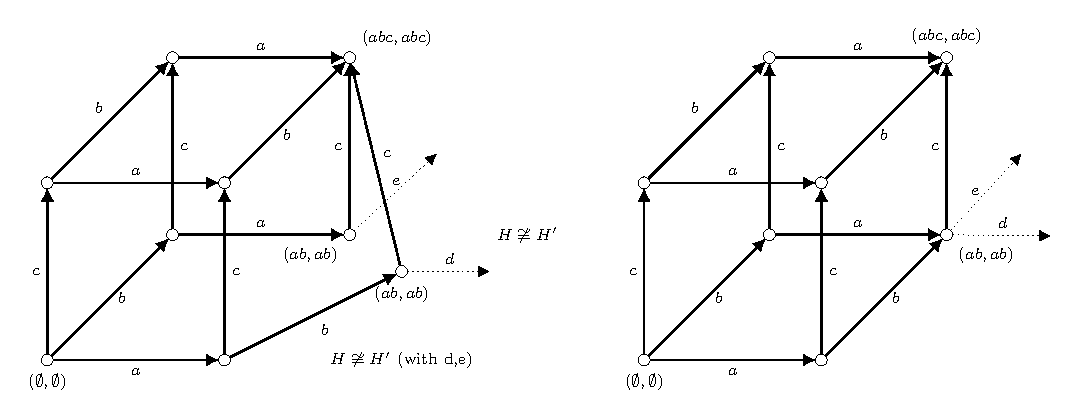
\includegraphics[scale=0.9]{Figures/5.Relationship-with-other-models-of-true-concurrency/broken_box(figure_6_left)/HDA-broken-box.pdf}
            \captionof{figure}[Broken box]{Example of sculptures, with ST-configurations as labels, and higher-dimensional automata representing the broken box example. The higher-dimensional automata (left) is not a sculpture, while the higher-dimensional automata (right) is a sculpture. We also see the higher-dimensional automaton (left) is not isomorphic to the higher-dimensional automaton (right). Since, the higher-dimensional automaton (left) has a split corner and the higher-dimensional automaton (right) is a nicely shaped cube.}
            \label{fig:HDA-broken-box}
        \end{figure}
    
        The example was of two computer scientists $A$ and $B$ travelling from one end of the podium to the other. Their task was to perform the actions $a$ and $b$, respectively, of crossing a line on the podium. Due to strategic placing of obstacles, the only place where this was possible was at a narrow opening between the obstacles that had room for only one of the scientist $A$ and $B$ at a time. This made the action $a$ and $b$ mutually exclusive, in the sense that they could not occur simultaneously.
    
        A third computer scientist $C$, was assigned the task $c$ of removing an obstacle that caused the bottleneck to exist. The action $c$ was executed causally independent of $a$ and $b$, that is, a and b are concurrent. The actions $a$ and $b$ were mutually exclusive only until $c$ occurred, after which they became causally independent.
    
        Finally, a fourth participant was assigned the task of making a statement when $a$ and $b$ had both occurred before the action $c$ started. This statement was going to be $d$ in case $A$ passed the bottleneck before $B$ did, and $e$ in case $B$ passed the bottleneck before $A$ did. Hearing this statement would prevent computer scientist $C$ from carrying out action $c$.
    
        The higher-dimensional automata (left) is not a sculpture, while the higher-dimensional automata (right) is a sculpture. We also see the higher-dimensional automaton (left) is not isomorphic to the higher-dimensional automaton (right). Since, the higher-dimensional automaton (left) has a split corner and the higher-dimensional automaton (right) is a nicely shaped cube.
    \end{example}
    
    \begin{theorem}[A non-sculpture]
        \label{th:non-sculpting}
        The $\HDA$ from Example \ref{exp:hda-broken-box} is not a sculpture.
    \end{theorem}
    
    \begin{proof}
    To show that the broken box cannot be sculpted we apply the labelling strategy described above.
    First we apply the unfolding procedure \hintost\ and for the two problematic corner states $q_{0}^{1}$ and $q_{0}^{2}$ we obtain the following ST-configurations $\hintost(\pi_{1})=(\{q_{1}^{1},q_{1}^{4}\},\{q_{1}^{1},q_{1}^{4}\})$ respectively $\hintost(\pi_{2})=(\{q_{1}^{2},q_{1}^{3}\},\{q_{1}^{2},q_{1}^{3}\})$, where $\pi_{1}$ is the lower rooted path ending in $q_{0}^{1}$ and $\pi_{2}$ is the other lower path ending in $q_{0}^{2}$.
    
    The second step is to apply the minimal equivalence \eventEquivHDAs, since this is required for any HDA. Indeed, if a HDA can be sculpted, then any cell of higher concurrency would be mapped to a unique cell in the bulk; in particular, each square from the HDA is mapped to a square in the bulk. Since we identify events in the bulk as opposite sides of bulk squares, then in the HDA any transitions opposite in a square would need to also be considered equivalent (this is what the minimal equivalence is doing).
    
    Now applying \eventEquivHDAs\ on our example equates $q_{1}^{1}\eventEquivHDAs q_{1}^{3}$ because of the three squares, front, top, back, which share the sides labelled with $a$ in the figure. (Transitivity of the equivalence was applied.)
    The same argument equates $q_{1}^{2}\eventEquivHDAs q_{1}^{4}$, this time going through the squares left-side, top, right-side.
    
    We now see that through $\rho_{\eventEquivHDAs}$ we have labelled both $q_{0}^{1}$ and $q_{0}^{2}$ with the same label $(\{[q_{1}^{2}],[q_{1}^{3}]\},\{[q_{1}^{2}],[q_{1}^{3}]\})$, made of equivalence classes.
    
    However, for a sculpture we cannot have two cells labelled the same. If an HDA can be sculpted, then we can find an embedding into a bulk. The embedding is by definition injective, meaning it maps two different HDA cells into two different bulk cells. But in the bulk each cell has a unique name in the canonical naming, as either a Chu-label or as an ST-configuration.
    \end{proof}
    
    There are more examples of non-sculptures, such as Figure \ref{fig:Unfolding-HDA}. The figure is also not representable as ST-structures and is not a sculpture. Both this example and Example~\ref{exp:hda-broken-box} are HDAs which are also their own unfoldings.